\documentclass[]{report}

\usepackage{amsfonts}
% or
\usepackage{amssymb}
\usepackage{amsmath}
\usepackage{minted}

\usepackage{xcolor}
\usepackage{color}
\usepackage{multicol}
\usepackage{tasks}
\usepackage{hyperref}
\usepackage{mathtools}

\usepackage[cc]{titlepic}
\usepackage{pseudocode}

\usepackage{booktabs}
\usepackage{subfigure}

\usepackage[titletoc]{appendix}

%Options: Sonny, Lenny, Glenn, Conny, Rejne, Bjarne, Bjornstrup
\usepackage[Rejne]{fncychap}

\setlength{\columnseprule}{0.2pt}

\DeclareTemplateInterface{tasks}{default}{3}
{
	% option        : type      = default
	enumerate       : boolean   = false    ,
	label           : tokenlist           ,
	indent          : length    = 2.5em   ,
	counter-format  : tokenlist = tsk[a]) ,
	label-format    : tokenlist           ,
	label-width     : length    = 1em     ,
	label-offset    : length    = .3333em ,
	after-item-skip : skip      = 1ex plus 1ex minus 1ex
}

\usepackage[a4paper,left=2.9cm,right=2.9cm,top=3cm,bottom=2.5cm,headheight=110pt]{geometry}


% Title Page
\title{{\Huge Route optimization for a fleet of vehicles with temporal constraints} \\
\noindent\rule{4cm}{0.4pt}\\
Algorithmics Methods and Mathematicals Models \\
Prof. Albert Oliveras LLunell and Prof. Lu\'is Velasco Esteban\\
\noindent\rule{4cm}{0.4pt}\\
Master in Research and Innovation}
\author{Juan Francisco Mart\'inez Vera \\
{\tt juan.francisco.martinez@est.fib.upc.edu}}
\titlepic{
\includegraphics[width=100px]{./imgs/upc_logo.jpg}}


\begin{document}
\maketitle

\newcommand{\localtextbulletone}{\textcolor{gray}{\raisebox{.50ex}{\rule{.6ex}{.6ex}}}}
\renewcommand{\labelitemi}{\localtextbulletone}

\begin{abstract}
	Optimization problems can appear in almost all situations on life. There are specially important those ones that appears on the industry because if we can achieve an optimal solution, we will improve the efficiency of the industrial process and then get lower manufacturing cost. This improvement of the costs have an effect on the competitiveness of the companies and on the final quality of their products and there are always good news for the customers. The challeging part is that those kind of problem have a really high computational complexity therefore there are several methods to face with them. By one hand we have the, let's say, always-optimality methods that obtain the optimal solution but without taking into account the huge amount of time that it could imply. e.g. ILP\footnote{Integer Linear Programming}. By the other hand we have those methods that concerns about the execution time and are looking for a tradeof between the exeution time and the quality of the solution\footnote{The distance to the optimal}.
	
	In this pages will be shown this two approaches in order to get the optimal routes for a fleet of vehicles taking into account temporal constraints.
	
\tableofcontents
	
\chapter{Introduction}
	Optimization problems can appear in almost all situations on life. There are specially important those ones that appears on the industry because if we can achieve an optimal solution, we will improve the efficiency of the industrial process and then get lower manufacturing cost. This improvement of the costs have an effect on the competitiveness of the companies and on the final quality of their products. The challeging part is that those kind of problem have a really high computational complexity therefore there are several methods to face with them. By one hand we have the, let's say, always-optimality methods that obtain the optimal solution but without taking into account the huge amount of time that it could imply. e.g. ILP\footnote{Integer Linear Programming}. By the other hand we have those methods that concerns about the execution time and are looking for a tradeof between the exeution time and the quality of the solution\footnote{The distance to the optimal}.
	
	In this project has been developed an Integer Linear Programming model in order to optimize the routes for a fleet of vehicles with temporal constraints derived from the distance between locations and from the tasks that has to be done for every location. Also have been developed different meta-heuristic strategies in order to get results more efficiently in terms of exeuction time even if there are not the optimal but close enough. Finnaly comparisons in term of execution time and solution quality have been done. 
	
\section{Document structure}
	The structure of this document is the following: The problem definition is done in chapter \ref{ch:problem_definition}. Here it is explained the problem that is faced, which constraints is needed to take into account and what we want to optimize. At chapter \ref{ch:ilp_model} is explained the mathematical model that has been developed, i.e. the decission variables and also the constraints with a mathematical nomenclature. After this chapter, at chapter \ref{ch:meta_heuristics} is explained how it has been used the heuristics approach in order to face with the problem, two meta-heuristics has been used: GRASP\footnote{Greedy Adaptative Search Procedure} and BRKGA\footnote{Biased Random-Key Genetic Algorithm}. After perform several executions for those approaches, a comparison in terms of time and quality of the result is done at chapter \ref{ch:comparison}. Finnally conclusions of the project are explained at chapter \ref{ch:conclusions}
\end{abstract}

\chapter{Problem definition}\label{ch:problem_definition}
\section{Description}
We have been asked to help one logistic company in the design of the daily routes of its fleet of vehicles. The workload for every day consist in some tasks that have to be done at a different locations, therefore, the problem is to identify the optimal routes for the minimum number of vehicles in order to perform all the work in time, i.e. starting at 8 a.m. and finalizing before 8 p.m. 

For that purpose we are given a set of locations and a start location $l_{s}$ where all the vehicles will start. For our point of view, the locations are not needed at all but we need the distance in terms of time between all of them. Because that we will be provided by the $dist_{l_{1},l_{2}}$ input data.

As is already mentioned, in every location (but not in $l_{s}$) there is a task that has to be done, then, also the information about how many time is needed for every task is provided as input data. We are talking about $task_{l}$.

Finally one more constraint is imposed by this logistic company. Every task has to be done but can not be started at any hour of the day. There is a temporal windows for every task that describes when an specific task can be started. This windows consists on a lower boundary $min_{l}$ and on a upper boundary $max_{l}$. Then the starting time can not be before $min_{l}$ and after $max_{l}$.

Considering that the company has an unlimited number of vehicles, the goal of the project is to find the minimum number of vehicles needed to visit all locations and perform all tasks, and define their routes. Given two solutions with the same number of vehicles it is preferred the one in which the latest vehicle arrives at its final destination sooner.

\section{Formal definition}

In this section is defined how the problem will be managed, also the input variables, the constraints and the objective function. This is a formal definition, therefore is implementation independant. These definitions have been used both for ILP and for meta-heuristics.

\subsection{A relaxed TSP with temporal constraints}\label{ss:relased_tsp}

This problem has been formally defined as a relaxed TSP\footnote{Travel Salesman Problem} with temporal constraints. It is relaxed because allows more than one cycle, i.e. more than one travel salesman (vehicle), and it is with temporal constraints because in addition to the usual weighted edges (routes) in the original TSP, we have temporal windows and tasks times for every node (location). The key point is that all the cycles in the graph, i.e. all routes, \textbf{must imply the $l_{s}$}.

This point of view allows to manage this problem without taking into account vehicles. The number of vehicles will be, in fact, the number of cycles in the solution.

As in TSP we can represent the towns and all routes as a directed weighted complete graph, then, we can describe a route of every vehicle by mean of a set of edges that describes a cycle. Remember that the cycle must implie the $l_{s}$ node.

The definition of the graph is defined by the below expression. Is important to mention that the cardinal of the $A$ set is like that because the distance of the travel from location a to location b could be different than the travel from b to a because the roads or whatever else.
$$G=(V,A) \quad where \quad \text{V: set of nodes, A: set of directed edges}$$
$$|V|=n, \text{being n = number of locations} \quad |A|=n^{2}-n$$

Now, let's define the set the whole possible cycles in the graph as $C$ where every cycle is defined as a subset of edges that fulfill all the conditions to be a cycle. Then, the set of all possible vehicles $VH \subset C$ are all the cycles that imples the $l_{s}$ as is described in the next expression:
$$vh \in VH \Leftrightarrow \exists a \in vh \text{ s.t. } a_{source} = l_{s} \lor a_{destination} = l_{s}$$

We can describe a set of potential solutions for the problem $PS \subset VH$ as all of subsets of $VH$ that cover all the locations without repeat any one of them. Those are potential solutions because for the moment we have not token into account the temporal constraints. Finally, the set of feasible solutions will be $S \subseteq PS$. And the challenging point is to get the optimal solution from this set.

\subsection{Input data}

According the definition, this variables are provided and describes a single instance of this problem. The following list describe all the input data that is provided. In order to improve the understanding, the input data have been split into two subsets. By one hand all data related to the graph stuff, and by the other hand the input data related to temporal restrictions.

\subsubsection{Graph input data}\label{sss:graph_constraints}
This input data is used in order to build up the graph that represents the problem and has been described several lines above. On next lines this input data is showed and explained.

\begin{itemize}
	\item \textbf{Number of locations} that the vehicles have visit. From here we can define the $V$ set that is the nodes set of the graph that are in fact the set of locations.
	$$
	n \in \mathbb{N}
	$$ 
	\item \textbf{Starting location} where all vehicles are placed at the beginning of times.
	$$
	l_{s} \in V
	$$
	\item \textbf{Distances} in minutes from one locations to the other. This data form the $A$ set because it is the weights for the edges for our completed directed and weighted graph. Note that when $a=b$, then $dist_{l_{a},l_{b}}=0$
	$$
	dist_{l_{a},l_{b}} \in A \quad \forall l_{a},l_{b} \in V
	$$
	Could be said that this is a temporal data but as this data is also needed to build up the graph, and is present on the original TSP as well, is prefered to be here.
\end{itemize}

\subsubsection{Time constraints input data}
This input data is used in order to build up the time constraints needed for the problem definition. On next lines this input data is shoed and explained.

\begin{itemize}	
	\item \textbf{Lower boundary} for the temporal windows for every location. It indicates from when a task can be executed. If one vehicles arrives before this time, it must wait. The temporal unit are the minutes. This minimum windows can be at most 720 that is the journey time in minutes ($8h*60min/h = 720min$)
	$$
	min_{l} \in [0, 720] \quad \forall l \in V
	$$
	\item \textbf{Upper boundary} for the temporal windows for every location. It indicates until when a task can be executed. Take into account that does not have sense that $max_{l} < min_{l}$
	$$
	max_{l} \in [min_{l}, 720] \quad \forall l \in V
	$$
	\item \textbf{Time} that a task spends for every location.
	$$
	task_{l} \in [0, 720], \forall l \in V
	$$
\end{itemize}

\subsection{Constraints definition}\label{ss:formal_constraints_definition}

In this section are explained the fundamental constraints that are implementation independant. As well as with input data on the previous section, in order to improve the understanding, the constraints are splitted into two subsets, the graph constraint and the time constraints.

\subsubsection{Graph constraints}

These constraints are derived from the format description of the problem as a directed weighted graph. All the solutions that exists in set $VH$ (section \ref{ss:relased_tsp}) fullfil the graph constraints. Just for summing up, those constraints are
\begin{itemize}
	\item Every location has to be visited exactly one time. It means that all cycles in a solution must cover all nodes and can not share any node.
	\item All cycles in a solution must involve the starting location.
\end{itemize}

\subsubsection{Time constraints}\label{ss:time_constraints}
These constraints have to guarantee that the time restrictions are fullfiled. Those constraints are:
\begin{itemize}
	\item The arrival time to location $l$ must be less or equal $max_{l}$.
	\item The arrival time to location $l$ must be $max(arrivalTime, min_{l})$. It means that if one vehicle arrive before  $min_{l}$ it will wait.
	\item The total time of a cycle must be less than 720 minutes that is 8 hours.
\end{itemize}

Note that the arrival time to a location is the sumation of the previous location arrival time plus the task of the previous location plus the time spent in the path (the weight of the edge).

\subsection{Objective function definition}\label{ss:objective_function}

In order to get the optimal solution we need to clasify every solution by a number that can tell us the quality of every one of them. This number is provided by the \textbf{objective function}.

As the description of the problem said, we want to minimize the number of vehicles and when two solutions have the same number of vehicles, we want the solution that end the whole job before. We will need two variables for this purpose, by one hand, the number of vehicles, lets say $nVehicles$ and by the other hand the time when the last vehicle ends its job, lets say $lastArrival$. How to get the correct value for these two variable is implementation dependant and therefore will be explained on the next chapters.

The objective functions is described as:
$$ Minimize \quad nVehicles*M + lastArrival$$
In this expression, the $M$ is a big enough number. It is needed in order to priorize the solutions with less value for $nVehicle$. When two solutions have the same number of vehicles, then the important value is the $lastArrival$.


\chapter{ILP model}\label{ch:ilp_model}

ILP\footnote{Integer Linear Programming} is the first of the two methods that has been used in this project. This method is always concerned on having the optimal solution without taking into account the amount of computational resources needed. This model is developed in CPLEX and the model implemented is described at the next sections.

\section{Input data}

From chapter \ref{ch:problem_definition} we already know which is the data that is provided. Now we need them in an specific shape in order to deal with them in CPLEX.

\begin{itemize}
	\item \textbf{Number of locations} $n$ is declared as an integer as well as \textbf{starting location}
	
	$$n \in \mathbb{N}$$			
	$$l_{s} \in \mathbb{N} \text{ s.t. } 1 \leq l_{s} \leq n$$
	
	\item The \textbf{distances} are modeled as two-dimensional matrix of integers that have $n^{2}$ positions. If you take into account that the values on the diagonal of the matrix will not be taked into account, the total number of distances is $n^{2}-n$ as we have described in the previous chapter. The distance is expressed in minutes.

	$$dist_{a,b} \in \mathbb{N} \quad \forall a,b \in [0, n) \text{ s.t. } a \neq b$$
	
	\item The remaining data fields are related to the locations, because that they are defined as a vector on $n$ positions. Those data fields are \textbf{lower boundary} and \textbf{upper boundary} of the temporal windows and the time spent in a \textbf{task}. All of them are expressed in minutes.

	$$task_{i}  \in \mathbb{N} \quad \forall i \in [0, n) \text{ s.t. } i \neq l_{s}$$
	$$minw_{i}  \in \mathbb{N} \quad \forall i \in [0, n) \text{ s.t. } i \neq l_{s}$$
	$$maxw_{i}  \in \mathbb{N} \quad \forall i \in [0, n) \text{ s.t. } i \neq l_{s}$$
\end{itemize}

\section{Decision variables}\label{s:decision_variable}

The solution of the problem will be encoded in a certain way in a decission variable. The decission variables are not only used for get the final result but also for enforcing some situation with constraints. Those variables unlike input data ones, are not statics and can change their value in order to fulfil the constraints (section \ref{s:ilp_constraints}), as is just said, and in the same time in order to maximize or minimize the objective function (section \ref{ss:objective_function}). Therefore, even if the important numbers for the solution are two. The number of used vehicles and the time when the last vehicle done the work is needed a sort of other decision variables. In the next list is presented a relation of the defined decision variable for model.

\begin{itemize}
	\item The \textbf{tracked} variable. It is a $n \text{x} n$ matrix and keep information about whether a path from location $n$ to location $n2$ is taken, i.e. keep information about which edges are on the solution. It is needed in order to control the number of input and output edges for every location, i.e. to control the correctness of the cycles and for calculate the time spent in a route by determining which paths have been taken and which ones not.
	
	$$tracked_{a,b} \in \mathbb{B} \quad \forall a,b \in [0, n) \text{ s.t. } a \neq b$$
	
	\item In order to build the temporal constraints that we have at section \ref{ss:time_constraints} we need information about when a vehicle arrives to a location. Because that the \textbf{arrivingTime} decision variable has been defined. It is an n-vector that keeps the arriving time for all locations (nodes) in minutes.
	
	$$arriving_{i} \in \mathbb{N} \quad \forall i \in [0, n) \text{ s.t. } i \neq l_{s}$$

	The starting location will not have arriving time, i.e. it will be always 0. The reasons are explained at section \ref{s:ilp_constraints}.
	
	\item One of the most important decision variables is the numbers of vehicles needed. \textbf{nVehicles} keep the number of vehicles in the solution.

	$$nVehicles \in \mathbb{N} \text{ s.t. } 1 \leq nVehicles \leq n$$
	
	On the best case, we only will need one vehicle but in the worst one we will need as much vehicles as locations.
	
	\item The other really important value for our result is the end time of the last vehicle. \textbf{lastDone} have the time in minutes of the last arrival vehicle.
	
	$$lastDone \in \mathbb{N}$$
	
\end{itemize}

%\section{Objective function}\label{s:ilp_objective_function}

\section{Constraints}\label{s:ilp_constraints}

For an ILP model the constraints part is the most important part, or at least the most tricky part. They are defining the solution space and because that we need to be careful in order to try to limit as much as possible but without prune some solutions and forbidding CPLEX to find a feasible solution when it exists.

The constraints below, as in section \ref{ss:formal_constraints_definition} have been separated into two sets. By one hand, the graph constraints and by the other hand, the time constraints.

\subsection{Graph constraints}

This constraints are the ILP version of the constraints defined at section \ref{sss:graph_constraints}.

\begin{itemize}
	\item The first constraint is worried about the fact that every location has to be visited exactly one time. For this purpose the \textit{tracked} decision variable is used. There is one special case where the number of visits for a location must be one or more. This special case will be the starting location because we want that all cycles involve it, therefore it will be visited at least one time.

	$$\sum\limits_{j \in V} tracked_{i,j} = 1 \quad \forall i \in V \text{ s.t. } i,j \neq l_{s}$$
	$$\sum\limits_{i \in V} tracked_{i,l_{s}} \geq 1 \quad \text{ s.t. } i \neq l_{s}$$
	
	The key point in this constraint is that we are counting the ingoing edges for all locations. 
	
	% TODO: Mirar si es posible simplificar esta constraint para que solo se garantice
	% TODO: que el numero de ingoing edges y outgoing edges sea igual en la starting location
	% DONE: No se puede. Si se cambia no funciona nada.
	
	\item From the previous constraint, we can ensure that every location just will have one ingoing edges but we are not ensuring anything about the outgoing edges. For cycles we want to ensure that there is only one outgoing edge for all location except for the starting one, that must be same outgoing edges as ingoing ones. Then, the sumation of outgoing edges must be equal as the ingoing edges for all locations.
	$$\sum\limits_{j \in V} tracked_{i,j} = \sum\limits_{k \in V} tracked_{k,i} \quad \forall i \in V $$
	$$ $$

	% TODO: Mirar si esta constraint se podria quitar. El hecho de que todos los ciclos
	% TODO: tengan que implicar la startlocation deberia ser suficiente
	% DONE: No es necesaria y de hecho mejoramos el tiempo de ILP si la eliminamos
	
	\item One desirable constraint is that we want to avoid the cycles that just imply one location. The point for this constraint is that we are enforcing 0 on the diagonal of the tracked matrix. As we will see later, since we are enforcing that all cycles must imply the startLocation, this constraint is not needed at all.

	$$ \sum\limits_{i \in V} tracked_{i,i} = 0 $$
	$$ $$

\end{itemize}

The constraints above are ensuring that our solution will contain cycles, and those cycles will visit all locations. Also is ensuring that all cycles are independant betweem them. The important thing that those constraints are not ensuring is that all cycles implies the starting location. This requirement will be fulfilled by time constraints as you will see on the next section.

\subsection{Time constraints}

This is the ILP implementation for the constraints defined at section \ref{ss:time_constraints}. As you will see below, this constraints are not enough, so some other have to be defined.

\begin{itemize}
	\item As we have seen at section \ref{s:decision_variable} just with the obvious decision variables is not enough in order to maintain all the constraints of times fulfilled. Because that {\tt arrivingTime} decision variable is needed. Since we have this variable is needed to constraint it, otherwise it will take whatever value. At every position of this vector we want to have the arriving time for the location with a determined id. If we think a little bit, there is one location that we already know its arriving time, this is the start location, and its arriving time should be zero and this constraint is enforcing this. This constraint is more important that it seems in principle. The implications are explained at section \ref{ss:arriving_time_0_implications}.
	
	$$ arriving_{l_{s}} = 0 $$

	\item Continuing with the arriving time, we also want good values for the rest of locations. In this constraint the arriving time for every locations is computed as the arriving time of the previous location plus the task done in that location plus the distance in minutes of the path that connects this pair of locations. Then, we must use the distances input data and also the decision variable {\tt tracked} in order to know which is previous location of the one that we are restricting.
	
	$$ \sum\limits_{i \in V} arriving_{j} \geq (arriving_i + task_i + distance_{i, j}) - (M*(1-tracked_{i, j})) \quad \forall j \in A \text{ s.t. } j \neq l_{s}$$
		
	For this equation, $i$ means the source location and $j$ means the destination. Take into account that we are avoiding the constraints for the $l_{s}$ because we are already restricting it to $0$ with the constraint above.
	The key point is that when the path from $i$ to $j$ is done (tracked is True) then we have a strong constraint\footnote{The constraint is great or equal because the arriving time could be greater than that if the vehicle must wait because the $minw$.}. By the other hand, if the path is not token then this is so soft constraint, in fact this is not restricting anything.
	
	\item This next constraint is concerned about the minimum windows arriving time. The point is that if the vehicle arrives before the minimum time, then it has to wait. The way to do so is restricting that the arriving time will be at least the minimum window. It is in fact a waiting.
	
	$$\sum\limits_{i \in V \text{ s.t. } i \neq l_{s}} arriving_{i} \geq minw_{i}$$
	
	\item And what about $maxw$? This constraints avoid those solutions that does not fulfil the window time requirements.
	
	$$\sum\limits_{i \in V \text{ s.t. } i \neq l_{s}} arriving_{i} \leq maxw_{i}$$
	
	\item Until here the model has been concerned about having good values for this, let's say, internal decision variable but what about the really important ones?. In this constraint we are ensuring a good value for the $nVehicles$ variable. In this model the number of vehicles are the number of cycles, so we just have to count how many cycles we have. To do so, an easy way is just count how many ingoing or outgoing edges we have for the start locations.
	
	$$nVehicles = \sum\limits_{i \in V \text{ s.t. } i \neq l_{s}} tracked_{l_{s}, i}$$
	
	\item The last part of this model is to ensure that the whole work is done before the end of the working day. To do so we need to have a good value for the $lastDone$ variable. In this model $lastDone$ is calculated by getting the arriving time for all of the locations that have an outgoing edge to start location, for every one of them do the summation of the task and the distance to start location and then get the biggest value.
	
	$$ \sum\limits_{i \in V} lastDone \geq (arriving_i + task_i + distance_{i, l_{s}}) - (M*(1-tracked_{i, l_{s}}))$$
	
	\item To end with this section, the last constraint is forbidding the working days over the eight hours (720 minutes).
	
	$$ lastDone \leq 12*60$$


\end{itemize}

\subsection{Avoiding cycles w/o starting location for free}\label{ss:arriving_time_0_implications}

At section \ref{ss:relased_tsp} has been explained how a vehicle is in fact a cycle. The important point is that all cycles represents all vehicles needed in our model and they must imply the start location. As you can see at section \ref{s:ilp_constraints} there is no explicit constraint that enforce this situation, so how it is actually  working?

Imagine a situation in which one we have two locations in a cycle and no one of them are the starting. And now take into account the way this model is enforcing a good value for the arriving time for locations. Is not possible to have an arriving time in any of them because there is not a fixed value, so the arriving time for both of them will be undefined, in other words, is not a solution.

By enforcing the arriving time to $0$ at starting location we are providing an exit point where all locations can go. Therefore, no cycle w/o starting location will form part of a valid solution, i.e. All the cycles of a valid solution will imply the starting location.

\chapter{Meta-heuristics}\label{ch:meta_heuristics}

In this chapter are explained via pseudocode the two meta-heuristics used for solve the problem. Only the most important parts will be shown, ignoring the rest of the code.

For GRASP the constructive phase and local search algorithms will be explained and for BRKGA, the chromosome structure and the decoder.

Just mention that the shape of the results for the meta-heuristics are the same as for ILP, that is the shape that has been described at section \ref{ss:relased_tsp}. It is a set of cycles, i.e. a set of paths

\section{GRASP implementation}
\subsection{Costructive phase}
This meta-heuristic has a constructive phase that is concerned to build up a feasible solution. This phase is not deterministic because the randomization done on the candidate pick process. It means that for every execution, different solution could be emerge\footnote{For $\alpha \neq 1$}. This part is based on a randomized greedy algorithm, so a greedy function is also needed.

You can see the constructive phase into two pseudo-codes. The constructive phase itself is at psheudcode \ref{pc:constructive_phase}. But in order to understand better what the developed heuristic is doing, you can see how the candidates set is generated at pseudocode \ref{pc:construct_cl}.

The essential idea is that a vehicle is moving through locations one after the other until it can not go to the next one because the time restriction. In this case, it returns to the $l_{s}$. Notice that at candidate generation is checked if moving to this next location there is a possibility to return to $l_{s}$, if not it is not considered a candidate.

\subsection{Local search}\label{ss:local_search}
The other part that will be shown is about the local search. Once the constructive phase ends up with a solution, eventually it is the optimal, but usually it is not. In order to improve the solution a neighbourhoods of the constructive phase solution, i.e. near solutions will be searched. This phase is called local search. Two neighbourhoods have been developed. The exchange and the reassignement. You can see the first one at pseudocode \ref{pc:exchange_neighbourhood} and the second one pseudocode \ref{pc:reassignement_neighbourhood}.

\subsubsection{Exchange neighbourhood}

This neighborhood is formed by all near solutions from the solution done by the constructive phase that differenciates with it because there is one location for one vehicle that has been changed for other location of other vehicle. Notice that searching in this neighborhood will not bring us a better solution in terms of number of vehicles but just in terms of final arrival time.

\subsubsection{Reassignement neighbourhood}

In this case, the differences between the solution at constructive phase and the solution on this neighbourhood is that one of the locations of one vehicle is not visited by this one but by other one. Notice that in this neighborhood is possible that we can have both, a better solution in terms of number of vehicles and in terms of final arrival time.

\subsection{Greedy function}
Finally, an important function for this meta-heuristic is the greedy function. This greedy function is giving us information about the quality of a candidate in order to decide if this candidate should be part of the solution or not. In this case, the greedy value depends on the characteristics of the path\footnote{The candidates are not locations but paths}, the characteristics of the locations that this path connects and also on the progression of the travel, i.e. on the travel time. 

$$ q(c, TravelTime) = TravelTime - distance(c) - minw(destination(c)) + task(source(c))$$

This greedy function is trying to give more importance to those candidates that implies less waiting time, i.e. it is trying to maximize the efficiency of the solution.

\begin{pseudocode}{grasp constructive phase}{\alpha, Paths, Locations}
\label{pc:constructive_phase}
	S \GETS \varnothing\\
	LastLocation \GETS l_{s}\\
	VisitedLocations \GETS \varnothing\\
	\\
	\WHILE \NOT size(VisitedLocations)=n-1 \DO
	\BEGIN
		TravelTime \GETS tavelTime(S)\\
		\COMMENT{The candidates are not locations but paths}\\
		C \GETS ConstructCL(LastLocation, TravelTime, VisitedLocations)\\
		\IF size(C) = 0 \THEN
			\RETURN{infeasible}\\
		
		\\
		\COMMENT{Notice that q(c) returns the greedy value for candidate c.}\\
		q_{min} \GETS min(q(c, TravelTime) \quad \forall c \in C)\\
		q_{max} \GETS max(q(c, TravelTime) \quad \forall c \in C)\\
		RCL \GETS {c \in C \text{ s.t. } q(c, TravelTime) \leq q_{min} + \alpha * (q_{max} - q_{min}) }\\
		\text{select } c \in RCL \text{ at random }\\
		\\
		S = S \cup {c}\\
		\IF destination(c) \neq l_{s} \THEN
			VisitedLocations = VisitedLocations \cup destination(c)\\
		LastLocation \GETS destination(c)\\
	\END\\
	\\
	\COMMENT{The return path to the start location for the last vehicle must be added.}\\
	ReturnPath \GETS getPath(destination(c), l_{s})\\
	S = S \cup ReturnPath\\
	
	\RETURN S

\end{pseudocode}

\begin{pseudocode}{ConstructCL}{FromLocation, TravelTime, VisitedLocations}
\label{pc:construct_cl}
	C \GETS \varnothing\\
	paths \GETS pathsFrom(FromLocation)\\
	\COMMENT{Filter unattainable locations}\\
	\FOREACH c \in paths \DO
		\IF maxw(destination(c)) \geq TravelTime  + task(FromLocation) + distance(c)\THEN
			C = C \cup c\\	
	\COMMENT{Filter visited locations}\\
	\FOREACH c \in C \DO
		\IF destination(c) \in VisitedLocations \THEN
			C = C - c\\
	\COMMENT{Filter those locations that if go there is not possible to return to $l_{s}$}\\
	\FOREACH c \in C \DO
	\BEGIN
		path_{1} \GETS getPath(FromLocation, destination(c))\\
		path_{2} \GETS getPath(destination(c), l_{s})\\
		time_{path_{1}} = max(TravelTime, minw(FromLocation)) + task(FromLocation) + distance(path_{1})\\
		time_{path_{2}} = max(time_{path_{1}}, minw(destination(c))) + task(destination(c)) + distance(path_{2})\\
		\IF time_{path_{2}} > 720 \THEN
			C = C - c\\
	\END\\
	\\
	\RETURN{\text{sorted } C \text{ by q(c)}}
\end{pseudocode}

\begin{pseudocode}{ExploreExchangeNeighbourhood}{S, strategy}
	\label{pc:exchange_neighbourhood}
	\COMMENT{The solution is a set of edges. This set of edges can be organized as cycles (vehicles)}\\
	V \GETS vehicles(S)\\
	\text{sort } V \text{ by } ArrivalTime \text{ desc}\\
	\\
	\COMMENT{Get the most loaded vehicle}\\
	MLVehicle = V[0]\\
	MLVehicleLocations \GETS locations(MLVehicle)\\
	\text{sort } MLVehicleLocations \text{ by } task \text{ desc}\\
	\\
	\COMMENT{Now get the locations of the rest of vehicles sorted by task asc}\\
	restOfLocations \GETS \varnothing\\
	\FOREACH v \in vehicles(S) \DO
		\IF v \neq MLVehicle \THEN
			restOfLocations \GETS locations(v)\\
	\text{sort } restOfLocations \text{ by } task \text{ desc}\\
	\\
	bestSolution \GETS S\\
	\FOREACH highLoadedLoc \in MLVehicleLocations \DO
	\BEGIN
		\FOREACH lowLoadedLoc \in restOfLocations \DO
		\BEGIN
			neighboor \GETS generateExchangeS(highLoadedLoc, lowLoadedLoc)\\
			\IF feasible(neighboor) \AND quality(neighboor) > quality(bestSolution) \THEN
			\BEGIN
				\IF strategy = \text{``FIRST-IMPROVEMENT"} \THEN
					\RETURN{neighboor}
				\ELSE
					bestSolution \GETS neighboor\\
			\END
		\END
	\END\\
	\RETURN{bestSolution}
	
	
	
	
\end{pseudocode}

\begin{pseudocode}{ExploreReassignementNeighbourhood}{S, strategy}
\label{pc:reassignement_neighbourhood}
	\COMMENT{The solution is a set of edges. This set of edges can be organized as cycles (vehicles)}\\
	V \GETS vehicles(S)\\
	vehiclesByLoad \GETS \text{sort } V \text{ by } ArrivalTime \text{ asc}\\
	vehiclesByLocation \GETS \text{sort } V \text{ by } nLocations \text{ asc}\\
	\\
	bestSolution \GETS S\\
	\FOREACH lessnLocactionsVehicle \in vehiclesByLocation \DO
	\BEGIN
		\FOREACH path \in lessnLocationsVehicle \DO
		\BEGIN
			locationToReassign = source(path)\\
			\IF locationToReassign \neq l_{s} \THEN
			\BEGIN
				\FOREACH lessLoadedVehicle \in vehiclesByLoad \DO
					\IF lessLoadedVehicle \neq lessnLocationsVehicle \THEN
					\BEGIN
						\COMMENT{Try to inject the location to some place of vehicle route}\\
						\FOREACH pathWhereInject \in lessLoadedVehicle \DO
						\BEGIN
							\COMMENT{If path is A-B and location is C, then try to A-C-B}\\
							neighbor \GETS generateReassignementS(locationToReassign,\\
							\quad \quad \quad \quad pathWhereInject)\\
							\IF feasible(neighboor) \AND \\
							\quad \quad \quad \quad quality(neighboor) > quality(bestSolution) \THEN
							\BEGIN
								\IF strategy = \text{``FIRST-IMPROVEMENT"} \THEN
									\RETURN{neighboor}
								\ELSE
									bestSolution \GETS neighboor\\
							\END
						\END
					\END
			\END
		\END
	\END
\end{pseudocode}

\section{BRKGA implementation}

\subsection{Chromosome structure}

For this implementation, the chromosome will encode the order in which the locations are pushing to the solution, in fact is a factor for the greedy value. The decoder is behaving as a greedy algorithm but with some modification in order to work with the chromosome as you will see at section  \ref{ss:brkga_decoder}.

Then the chromosome will have as many gens as locations, and every gen will have a value from 0 to 1. This value is the weight that modify the order of the candidate set at decoder.

\subsection{Decoder}\label{ss:brkga_decoder}

Recapping, the greedy algorithm is based on the idea to bring for every candidate a value that means the quality of every one of them. This value is provided by the greedy function. For purely greedy algorithms, the candidates are sorted by this value and then the best one (the first one of the list) will be included on the solution. An evolution of greedy is GRASP that is randomizing the pick of a candidate with its RCL. This decoder is following the same idea. In this case, every gen is multiplied for the greedy value of the destination of every candidate (remember that the candidates are paths). It means that the gens are affecting to the position of the candidates in the candidates list. Once we have all the candidates sorted, the first one is picked. Notice that the decoder is deterministic. The randomicity in BRKGA is not in the greedy part but in the generation of mutants.

You can see the pseudocode of decoder at \ref{pc:brkga_decoder}

\begin{pseudocode}{ExploreReassignementNeighbourhood}{chromosome}
	\label{pc:brkga_decoder}
	S \GETS \varnothing\\
	LastLocation \GETS l_{s}\\
	VisitedLocations \GETS \varnothing\\
	\\
	\WHILE \NOT size(VisitedLocations)=n-1 \DO
	\BEGIN
	TravelTime \GETS tavelTime(S)\\
	\COMMENT{The candidates are not locations but paths}\\
	C \GETS ConstructCL(LastLocation, TravelTime, VisitedLocations)\\
	\IF size(C) = 0 \THEN
	\RETURN{infeasible}\\
	\\
	\COMMENT{getGen(chromosome, location) provides the value of the gen for location.}\\
	c \GETS min(q(c, TravelTime)*getGen(chromsome, destination(c)) \quad \forall c \in C)\\
	\\
	S = S \cup {c}\\
	\IF destination(c) \neq l_{s} \THEN
	VisitedLocations = VisitedLocations \cup destination(c)\\
	LastLocation \GETS destination(c)\\
	\END\\
	\\
	\COMMENT{The return path to the start location for the last vehicle must be added.}\\
	ReturnPath \GETS getPath(destination(c), l_{s})\\
	S = S \cup ReturnPath\\
	
	\RETURN S
\end{pseudocode}

\chapter{Tunning and Comparisons}\label{ch:comparison}

There are some interesting comparisons that can be do, not just compare ILP with meta-heuristics solutions. An interesting studies are for try to tune accuratelly the meta-heuristics parameteres. In this chapter you will see how those parameteres are tuned through an empirical reasoning. An study of the $\alpha$ value for GRASP is done at section \ref{s:tuning_alpha}. More parameters have to be taken into account for BRKGA, that are: percentage of elites, percentage of mutants, number of individuals, percentage on inheritage and number of generations. In this case some simplications have done in order to fulfil with the deadline. You can see this study at section \ref{s:tuning_brkga_params}. Finally, at section \ref{s:comparison} a comparison between ILP and meta-heuristics is done.

\section{Instances complexity factors}\label{s:complexity_factors}

Fisrt of all a little study has been done in order to know in a better way which factors made a problem, computational power hungry or not for ILP. A naive approach could be to say just the number of locations. But there are more factors that affects on the complexity of the problem. Since ILP is taking into account all the possible solutions and then get the best one, when you are providing to the ILP model an instance where almost all combinations can be done, it will take a lot of time. So, three principal factors have to be token into account.

\begin{itemize}
	\item Number of locations. Of course, as more locations we have, more combinations of routes can be done.
	\item The size of the time window. The time window is a good tool in order to prune options for routes. As more big is the windows of the locations more posibilities to move from one location to another the model has. As more little one, less posibilities to move.
	\item The distances between the cities. Also an obvious factor. As more scattered are the locations on the a bidimentional space, less jumps from one location to another can be done.
\end{itemize}

At plot \ref{img:time_vs_wsize} it can be seen the results for some experiments that are done in order to see the impact of the windows size. All these experiments are done with scattered distribution of locations. The conclusion is that when we have a little amount of cities, the windows size is not so important, but for bug amount of cities it affects a lot.

Has been decided to do this little study, that just take some minutes thinking on the problem, in order to end up with scaled instances for perform the experiments. We want complex enough inputs but not so complex that could imply more time that we have. To do so, some modifications in the {\tt InstanceGenerator} have done. Now you can decide the number of locations, of course, but also the maximum window and if the cities will be scattered on a big space or in a little one. The big space implies that the starting locations will be at the middle and the other will be as maximim at 360 minutes from it. The small space implies that the start location is placed randomly and then the maximum distance between all locatios is 360 (just the minutes that we need to go and return assuming task of 0 minutes).

\begin{figure}
	\caption{Time spent by ILP for different problem size for windows time at max 350 and 500}
	\label{img:time_vs_wsize}
	\centering
	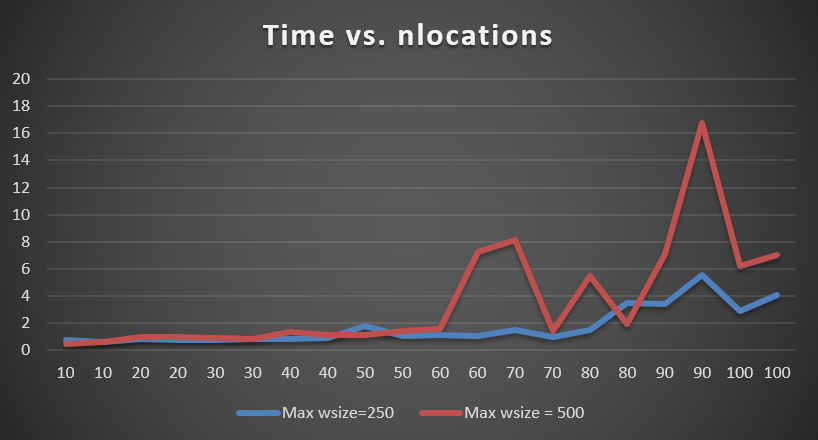
\includegraphics[width=0.9\textwidth]{./imgs/ilp_wsize_aggregated.png}
\end{figure}

In conclusion a tradeoff between number of locations, windows size and how to distribute the locations must be done. Since this point all the instances used for the executions have been generated taked into account those factors.

\section{Tuning $\alpha$ parameter for GRASP}\label{s:tuning_alpha}

On GRASP, a good tune of $\alpha$ parameter is a critical issue. When this parameter is 1 the met-heuristics becomes a completelly random algorithm. By the other hand when it becomes 0, the algorithms will behave as a purelly greedy one.

Some tests has be done with different number of locations for different $\alpha$. 20 tests are done. 4 test por every number of locations. And the number of locations as gone from 10 up to 100.

As you can see in figure \ref{img:grasp_alfa} the most suitable $\alpha$ for this problem is near $0,25$ then we will use this value for the next experiments.

This plot confronts the quality of the solution and the $\alpha$ parameter. For this experiment has been toked the best solution of the four experiment for each $\alpha$ and number of locations and compare the rest of the solutions whith same parameters which this one.

One interesting fact that also can be seen on the plot is that as we are incrementing the number of locations, the degradation because $\alpha$ is also increasing. An explanation for this fact is the synthetic instance generator. The instance generator developed for this project is just ensuring that you will have at least the basic solution that is have as much vehicles as locations. After ensure that it relaxes some data by randomizing values like task and time windows. When you have a little ammmount of locations this relaxation is not enough and the number of possible solutions is still near 1. Since the number of locations is incrementing, then the number of possible solutions is also incrementing and by get bigger $\alpha$ we are seeing those other solutions.


\begin{figure}
	\caption{Evolution of quality of solution changing $\alpha$ parameter.}
	\label{img:grasp_alfa}
	\centering
	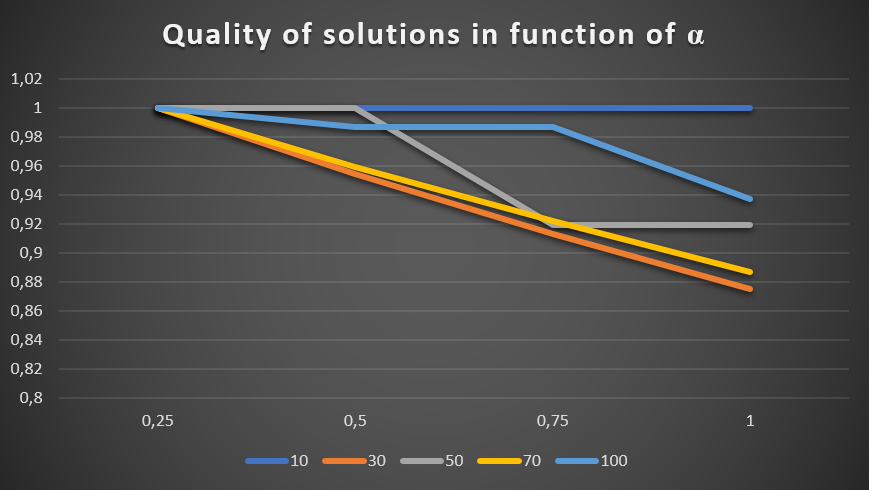
\includegraphics[width=0.9\textwidth]{./imgs/grasp_alfa_comparisons}
\end{figure}



\section{Tuning BRKGA parameters}\label{s:tuning_brkga_params}

For BRKGA the tuning is a little bit more difficult than for GRASP. Here we have five parameters to tune.
\begin{itemize}
	\item $nIndividuals$ Number of individuals in a poblation.
	\item $pElites$ Percentage of the poblation that becomes elite.
	\item $pMutants$ Percentage of poblation to generate as mutants.
	\item $pInheritanceElite$ Boundary value that decides if a gene is get from elite or from a normal individual on the crossover.
	\item $maxGenerations$ And finally the number of generation that we want to evolve.
\end{itemize}

In order to fulfil with the deadline of the project all the needed experiments are not done but just a little subset of them. It has been defined three different sets of parameters and every set has been executed over the same instances like the experiments for the GRASP at section \ref{s:tuning_alpha} from 10 to 50 locations.

Those four sets are:
\begin{itemize}
	\item Let's start with the configuration provided by default with the meta-heuristics framework. This configuration is: 
	\begin{itemize}
		\item $nIndividuals=nLocations/2$
		\item $pElites=0.2$
		\item $pMutants=0.15$
		\item $pInheritanceElite=0.7$
		\item $maxGenerations=3$
	\end{itemize}
	\item Now let's try incrementing the number of individuals. This experiment is trying the exploit the generation of mutants in order to leave of local optimals.
	\begin{itemize}
		\item $nIndividuals=nLocations$
		\item $pElites=0.2$
		\item $pMutants=0.15$
		\item $pInheritanceElite=0.7$
		\item $maxGenerations=3$
	\end{itemize}
	
	\item In this experiment is almost equal the previous one but doubling the number of elite individuals. 
	\begin{itemize}
		\item $nIndividuals=nLocations$
		\item $pElites=0.4$
		\item $pMutants=0.15$
		\item $pInheritanceElite=0.7$
		\item $maxGenerations=3$
	\end{itemize}

	\item  In this experiment is almost equal the previous one but doubling the number of elite mutants. 
	\begin{itemize}
		\item $nIndividuals=nLocations$
		\item $pElites=0.2$
		\item $pMutants=0.3$
		\item $pInheritanceElite=0.7$
		\item $maxGenerations=3$
	\end{itemize}
\end{itemize}

As you can see at figure \ref{img:brkga_experiments} the quality of the solutions are not changing at all. Only for the last input of 50 locations. Then we will use the first experiment parameters. The fact that there are not so many changes with the different parameters also could imply that the inputs are really constrained and encourage us to keep developing the {\tt InstanceGenerator} for try to relax a little bit more the inputs.

\begin{figure}
	\caption{Evolution of quality of solution for different experiments.}
	\label{img:brkga_experiments}
	\centering
	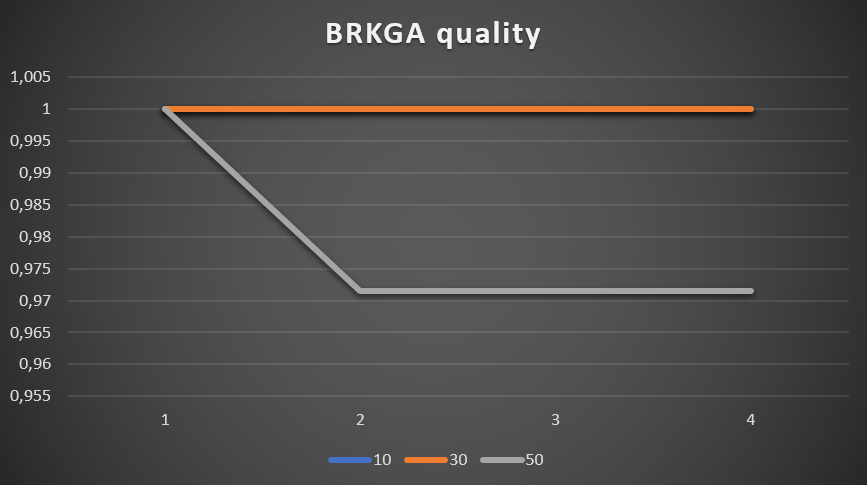
\includegraphics[width=0.9\textwidth]{./imgs/brkga_experiments}
\end{figure}

\section{Comparison: ILP vs meta-heuristics}\label{s:comparison}

Now, a comparison in terms of time and quality of the result will be showed up. The quality of a result is the distance to the optimum. Taking into account that the solution of ILP is always the optimum, just have been calculated the quality for the two metaheuristics.

The tricky part in order to do this comparison has been pick the correct instances. As it has been explained at section \ref{s:complexity_factors} get the correct instances is not just a matter of move over the different intances sizes in terms of number of locations. Because the randomness of the instance generation is difficult to get the perfect input for the experiment that you want to do even if you are controlling all the explained factors.

The used instances have been instances that have an increasing time in ILP. This is just to see what is the evolution of execution times of meta-heuristics and also the evolution of the quality of the solutions since the end of this section is to make comparisons, not denote the evolution of times vs. input sizes. Is because that you will see that the instances on the x axys are unsorted in terms of number of locations.

\subsection{Quality comparison}

At figure \ref{img:metaheuristics_quality_comparison} you can see the plot with the qualities of the solutions for four different instances. As is just said, the instances are not sorted by the number of locations but by the time spent in ILP because is considered that this time is a clear indicative for the complexity of the instance of the problem. Looking at the quality, it seems that as more number of locations we have, more further from the optimality the meta-heuristics are and this is the expected phenomena. Also another appreciation arise. Those values are saying us, at least for the different version for GRASP, that the complexity of an instance from the point of view of it is clearly correlated with the number of locations and it is saying that in fact its possible that the instances complexity factors described at section \ref{s:complexity_factors} are not aplying completely to meta-heuristics.

So, the conclusions for this comparison is that in general BRKGA is behaving better than GRASP. And for the different versions of GRASP, the best is GRASP+Reassignement. This is also as we are expecting because as has been explained at secion \ref{ss:local_search} scan on reassignement neighbourhood can end up a better solution by removing one vehicle. For the exchange neighbourhood this kind of improvement is not expected but just an improvement in terms of a better arrival time.

\begin{figure}
	\caption{Comparison in terms of quality of the different applied meta-heuristics.}
	\label{img:metaheuristics_quality_comparison}
	\centering
	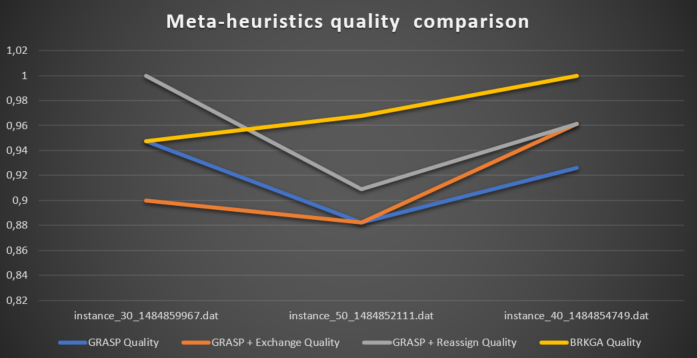
\includegraphics[width=0.9\textwidth]{./imgs/metaheuristic_quality_comparison.png}
\end{figure}

\subsection{Time comparison}

At figure \ref{img:ilp_metaheuristics_comparison} you can see the plot with the comparisons of execution times. Be careful for a fast conclusion just looking for lines, take into account that the y-axys is in a logarithmic scale. You can see, as was expected that ILP is the clear defeated because looking at figure \ref{img:metaheuristics_quality_comparison}, those times are not justified. The quality of the solutions are not so distant, so the efficiency (let's say $\frac{quality}{needed resources}$) of ILP, at least in these experiments is clearly below the efficiency of meta-heuristics.

About the meta-heuristics there are some things to mention. All the versions are paying the better quality with execution time. In fact the order is inverse than the order of the best meta-heuristic for quality. The differencies between GRASP+Exchange and GRASP+Reassign can be explained because the size of the neighbourhood that every one is scanning. Of course, the reassignement one is more bigger than the other.

Finnaly, the same appreciation like on the section above. It seems that the number of locations are strong correlated with the needed resources for meta-heuristics but not for ILP.

\begin{figure}
	\caption{ILP vs Meta-heuristics times comparison}
	\label{img:ilp_metaheuristics_comparison}
	\centering
	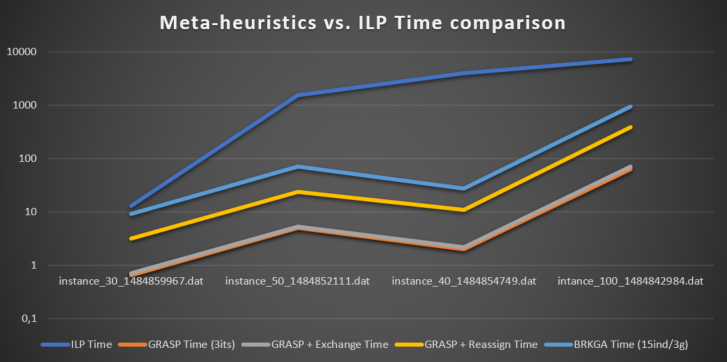
\includegraphics[width=0.9\textwidth]{./imgs/ilp_vs_metaheuristics_time_comparison.png}
\end{figure}

\chapter{Conclusions}\label{ch:conclusions}

In this project has been developed an ILP model and two meta-heuriscs in order to find out the optimal paths for a fleet of vehicles taking into account time constraint.

About the ILP has been really challenging to end up with a really simplified model that does not know anything about vehicles. This simplicity allows to model to work with two-dimensional matrix instead of three-dimensional ones that will imply more time resources for get the optimal value. Also an extra effort has been done for give it flexibility in terms on confire where the starting location is. And keeping on with the simplicity idea, this model enforce the generation of cycles without an explicit constraint. This is because some time constraint as has been explained. It was for free because the idea was to work on this constraint later.

About meta-heuristics, has been also so challeging to end up with a reasonable greedy function, that is in fact the hearth of all applied metaheuriscis here.

But the more challenging part has been to get a good inputs for the experiments. Has been so difficult because the complexity is not only a matter of number of locations but also another factors. The difficulty was because it can be generated two different instances with the same number of locations and one of them finalize at seconds and the other take ours until the computer run out of memory. Finally some good inputs has been picked by tunning the {\tt InstanceGenerator}.

About the results they are so satisfactory because they are approximatelly as I was expecting. Anyway has been a surprise for me the power of the meta-heuristics. They can achieve a results really close to the optimal in a few minutes or even seconds while ILP is taking even hours. One commentary here for the executions of ILP. There are some situacions where it conversge very rapid to a less than 10\% but it is running for hours just for this 10\%. Maybe a more fine tunning of cplex in order to configure the minimum quality of results will save a lot of computational time. 

\section{Future work}

More studies in order to get the optimal parameters for the meta-heuristics have to be done. Also one limitation of the experiments done in this project is that all the instances are generated with synthetic data, it means that of course they are biased by the nature of the generator. So it could be interesting to work with real data.

\newpage

\begin{appendices}
	\chapter{Instance generator}
	For testing the ILP model and the meta-heuristics and perform the experiments an instance generator has been done. This instance generator allows us to generate feasible inputs. You will see the input generator script in attached with this report.
	
	The usage of the script is:
	\begin{center}
		{\tt python ./InstaceGenerator.py <nlocations> <maxwinsize> <SCAT | GATH>}
	\end{center}
	
	The different parameters are:
	\begin{itemize}
		\item {\tt nlocations}: For sure, the number of locations that you want on the instance.
		\item {\tt maxwinsize}: The maximum sizes of the time windows. It means that the size of the windows of all locations will be set randomly from 1 to this number.
		\item {\tt <SCAT | GATH>}: You must choice between scattered distribution or gathered. For scattered the nlocations-1 locations will be dispersed over a bidimensional are where the distance from the center to one corner is exactly $720/2$. Since the startLocations will be on the center of the area, there is ensuring that all distributions will end up with a feasible solution because always a vehicle can travel from startLocation to the most remote location. For the gathered distribution the distance of the diagonal is $720/2$ and all locations are distributed randomly. It means that the maximum distance between two locations will be 360.
	\end{itemize}
	
	Finally, the script will generate an instance with the name:
	\begin{center}
		{\tt instance\_<nlocations>\_<random\_seed>.dat}
	\end{center}
	
	\chapter{Result visualizer}
	
	As an extra work, a basic visualizer has been developed. It shows the results by reading the output of ILP (previously saved on a file). The representation of the result is with directed graph and also can be seen the arrival time for every locations. To see the graphical representation of a solution you must execute:
	\begin{center}
		{\tt python ./ResultVisualizer.py <file\_with\_dumped\_result.txt>}
	\end{center}
	There are some examples below:
	
	\begin{figure}[h]
		\centering
		\subfigure[Example 1]{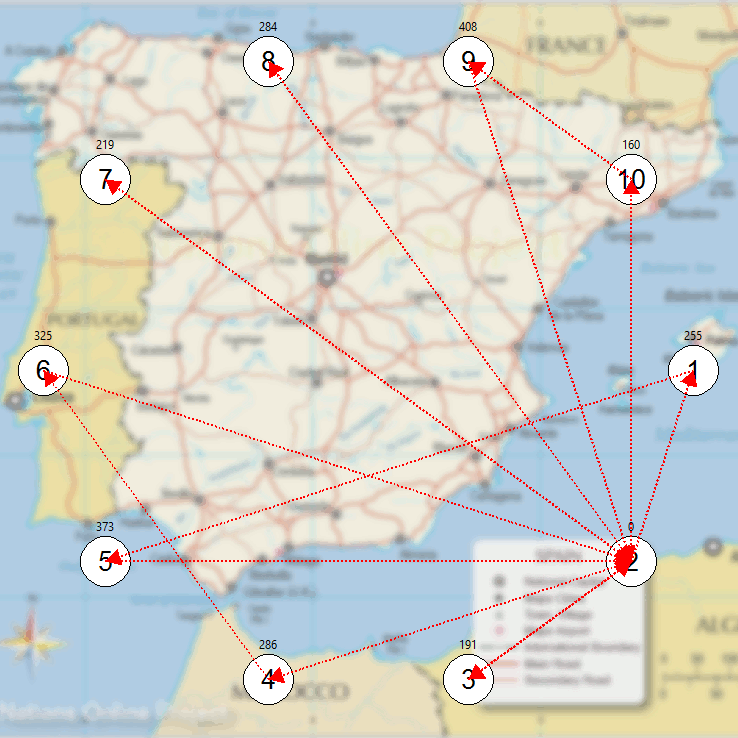
\includegraphics[width=0.30\textwidth]{./imgs/result_visualizer_example_1.png}}\hspace{15mm}
		\subfigure[Example 2]{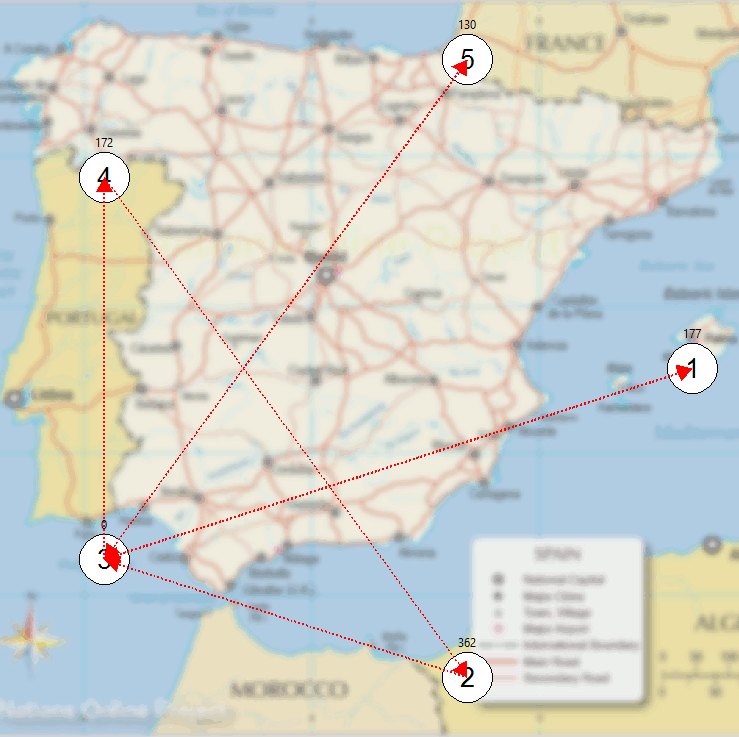
\includegraphics[width=0.30\textwidth]{./imgs/result_visualizer_example_2.png}}\vspace{5mm}
		\subfigure[Example 3]{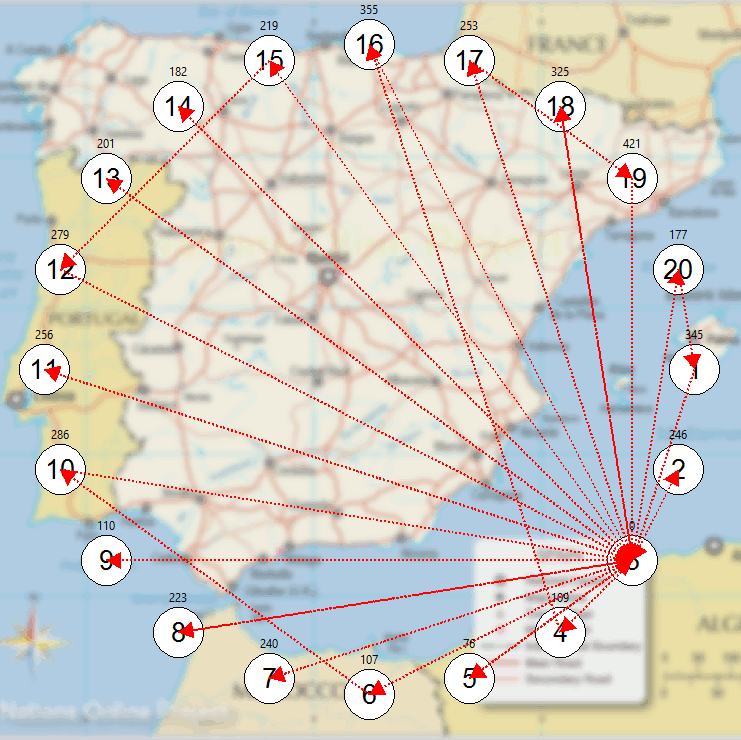
\includegraphics[width=0.30\textwidth]{./imgs/result_visualizer_example_3.png}}\hspace{15mm}
		\subfigure[Example 4]{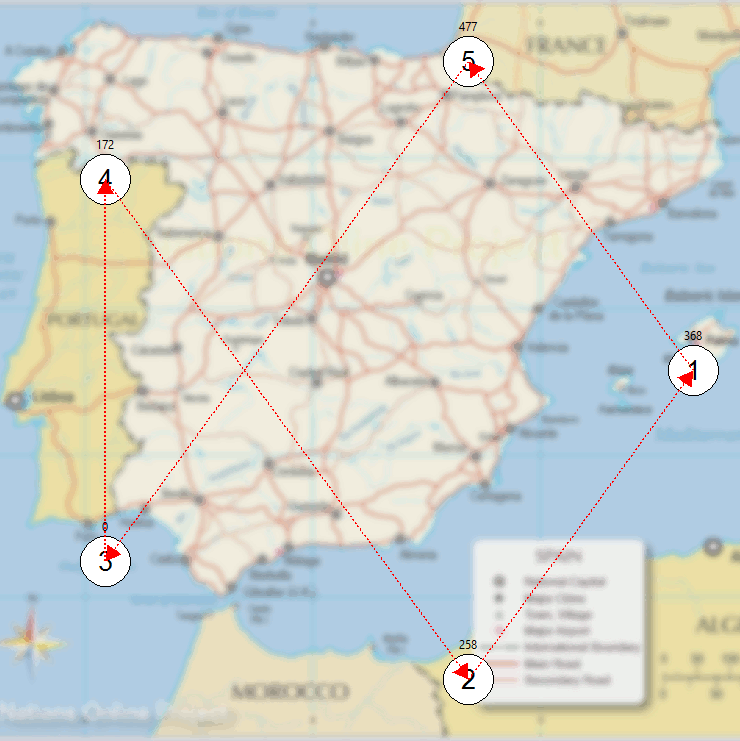
\includegraphics[width=0.30\textwidth]{./imgs/result_visualizer_example_4.png}}
	\end{figure}
\end{appendices}
	

\end{document}          
